\chapterauthor{Jeferson J. Lima}{Departamento de Informática (DAINF) \\Universidade Tecnológica Federal do Paraná (UTFPR)}
\chapter{Cinemática e Dinâmica de Robôs Móveis com Rodas}


\section{Introdução}\label{intro}
% 2. Cinemática e Dinâmica de Robôs Móveis com Rodas
% 	2.1 Cinemática Direta e Inversa
% 		2.1.1 Cinemática Direta e Inversa
% 		2.1.1 Cinemática de Robôs Móveis com Rodas
% 	2.2 Restrições de Movimento
% 		2.2.1 Sistemas Holonômicos
% 		2.2.2 Sistemas Não-Holonômicos
% 	2.3 Modelagem de Robô Móvel com restrições de Movimento.
% 3. Controle Moderno para Robótica Móvel
% 	3.1 Lyapunov-based Controle
% 	3.2 SDRE Controle
% 4. Eventos Não Deterministicos em Robótica Móvel
% 	4.1 Estimação de Estados
% 	4.2 Filtro Bayesiano
% 	4.3 Filtro de Kalman
% 		4.3.1 Filtro de Kalman Estendido

A humanidade é fascinada pelo movimento das rodas a milhares de anos, isso intriga até os dias de hoje, o homem moderno.
Na matemática há áreas específicas para descrever o movimento dos corpos, ou para o nosso interesse nesse capítulo, a cinemática dos robôs. 
Um modelo cinemático de um robô, com rodas ou pernas, descreve as relações geométricas entre que dão forma ao próposito deste robô.

Em resumo, os modelos cinemáticos estão relacionadas a como as velocidades dos elementos do robô interagem entre si e o espaço.

\section{Rotação, Translação e Transformação Homogênea}\label{rotacao}
 
Para representação de posicionamento e orientação de um sistema de coordenadas faz se necessário seguir a metodologia do sistema universal de coordenadas.

De acordo com \cite{craig2009introduction} uma vez estabelecido o sistema de coordenada como um vetor de posição $\mathbb{R}^{3 \times 1}$, composto pelas coordenadas $X,Y$ e $Z$, podemos então representar os operadores de rotação, translação e transformação homogênea como operações matriciais. Desta forma, um ponto ${}^A\mathbf{P}$ representa a distância ao longo dos eixos do plano $\{A\}$. Os elementos individuais de ${}^A\mathbf{P}$ podem ser visto pela equação \eqref{eq:cine1}.

\begin{equation}\label{eq:cine1}
    {}^A\mathbf{P} = \begin{bmatrix}
    p_x\\ p_y \\ p_z
    \end{bmatrix}.
    \end{equation}
    
    A representação gráfica de ${}^A\mathbf{P}$ pode ser vista na figura \ref{fig:cine1f}. 
    
    \begin{figure}[!ht]
    \centering
    \begin{tikzpicture}[scale=0.8]
    \node(p0) at (0,0){};
    \draw [->] (p0.center) --++(0,3) node[right] {$ Y_A$};
    \draw [->, rotate =120] (p0.center) --++(0,3) node[below] {$ Z_A$};
    \draw [->, rotate =240] (p0.center) --++(0,3) node[below] {$ X_A$};
    \draw [->] (p0.center) --++(2.5,0.5) node(B)[above,rotate=30] {${}^A\mathbf{P}$};
    \node at (-1.5,2.5) {$\{A\}$};
    \end{tikzpicture}
    \caption{Vetor em relação ao plano $\{A\}$}
    \label{fig:cine1f}
    \end{figure}
    
    Além da definição das coordenadas de um vetor, torna-se necessário definir a orientação desse corpo no espaço. O vetor definido por ${}^A\mathbf{P}$ pode ser rotacionado pela matriz de rotação $\mathbf{R}$, conforme a equação \eqref{eq:cine2}.
    
    \begin{equation}\label{eq:cine2}
    {}_A^B
    \mathbf{R} = 
    \begin{bmatrix}
    r_{11} & r_{11} & r_{11}\\
    r_{21} & r_{21} & r_{21}\\
    r_{31} & r_{31} & r_{31}\\
    \end{bmatrix}
    \end{equation}


    Na figura abaixo, a posição de ${}^A\mathbf{P}$ (sistema de referência global) em relação a ${}^B\mathbf{P}$ é encontrado através da multiplicação da matriz de ${}_B^A \mathbf{R}(\theta)$ (lê-se rotação do sistema de referência $B$ em $A$) pela posição de ${}^B\mathbf{P}$

    \begin{figure}[!ht]
        \centering
        \begin{tikzpicture}[scale=0.8]
            \node(p0) at (0,0){};
            \draw [->] (p0.center) --++(0,3) node[right] {$\hat Y_A$};
            \draw [->, rotate =120] (p0.center) --++(0,3) node[below] {$\hat Z_A$};
            \draw [->, rotate =240] (p0.center) --++(0,3) node[below] {$\hat X_A$};
            \draw [->, rotate =-10, gray] (p0.center) --++(1.5,2) node(A)[above,rotate=30] {${}^A\mathbf{P}$};
            \node(p1) at (6,1){};
            \draw [->, rotate =30, red] (p0.center) --++(0,3) node[right,rotate=30] {$\hat Y_B$};
            \draw [->, rotate =150, red] (p0.center) --++(0,3) node[below,rotate=30] {$\hat Z_B$};
            \draw [->, rotate =270, red] (p0.center) --++(0,3) node[below,rotate=30] {$\hat X_B$};
            \draw [->, rotate =20, red] (p0.center) --++(1.5,2) node(B)[above,rotate=30] {${}^B\mathbf{P}$};
        \end{tikzpicture}
        \caption{Vetor em rotação no plano $\{A\}$}
        \label{fig:vetor_rot}
    \end{figure}
    
    Abaixo segue um exercício numérico de fixação.

    \begin{shortbox}
        \Boxhead{Exercício de Fixação}
        Como exemplo, uma rotação $\theta$ de ${}^AP$ em torno do eixo $Z$ é descrita pela figura  \eqref{fig:vetor_rot}. 
        
        
        
        Pode-se observar que é adicionado uma coluna e linhas com zeros e uma nova linha em  \eqref{eq:cine3}, essa notação torna-se necessária pois será posteriormente apresentando o operador de translação.

        \begin{equation}\label{eq:cine3}
        {}^B\mathcal{P} = {}_A^B \mathbf{R}(\theta) {}^A\mathbf{P} = 
        \begin{bmatrix}
        \cos(\theta) & \sin(\theta) & 0 & 0\\
        \sin(\theta) & \cos(\theta) & 0 & 0\\
        0 & 0 & 1 & 0\\ 
        0 & 0 & 0 & 1\\
        \end{bmatrix}.
        \begin{bmatrix}
        {}^Ap_x\\
        {}^Ap_y\\
        {}^Ap_z\\
        1
        \end{bmatrix}
        \end{equation}
        \begin{center}
            Resposta:
    
\qrcode[height=0.8in]{
[-1,  0,  0,  0],
[ 0, -1,  0,  0],
[ 0,  0,  1,  0],
[ 0,  0,  0,  1]]
}
    \end{center}
    
    \end{shortbox}

    A rotação pode acontecer tanto em $x, y$ ou $z$, conforme é mostrado abaixo:

    \begin{equation*}
        \mathbf{R}_x(\theta) =
        \begin{bmatrix}
            1 & 0            & 0             \\
            0 & \cos(\theta) & -\sin(\theta) \\
            0 & \sin(\theta) & \cos(\theta)  \\
        \end{bmatrix} \text{, eixo $x$ fixo}
    \end{equation*}
    \begin{equation*}
        \mathbf{R}_y(\theta) =
        \begin{bmatrix}
            \cos(\theta)  & 0 & \sin(\theta) \\
            0             & 1 & 0            \\
            -\sin(\theta) & 0 & \cos(\theta) \\
        \end{bmatrix} \text{, eixo $y$ fixo}
    \end{equation*}
    \begin{equation*}
        \mathbf{R}_z(\theta) =
        \begin{bmatrix}
            \cos(\theta) & -\sin(\theta) & 0 \\
            \sin(\theta) & \cos(\theta) & 0 \\
            0            & 0            & 1 \\
        \end{bmatrix} \text{, eixo $z$ fixo}
    \end{equation*}

    Frequentemente o sistema de referência $\{A\}$ não coincide em nenhum coordenada de $\{B\}$, sendo assim, deve-se representar o deslocamento entre os planos. Esse deslocamento é chamado de translação, e dá-se pelo operador translacional $\mathbf{D}_A(q)$, onde ${}^A\mathbf{Q}$ representa uma translação entre os planos $\{A\}$ e $\{B\}$ e é expresso pela equação \eqref{eq:cine4}.

    \begin{equation}\label{eq:cine4}
    {}^A\mathbf{Q} =
    \begin{bmatrix}
    q_x\\ q_y \\ q_z
    \end{bmatrix}, \qquad \mathrm{e} \qquad
    \mathbf{D}_A = 
    \begin{bmatrix}
    1 & 0 & 0 & q_x\\
    0 & 1 & 0 & q_y\\
    0 & 0 & 1 & q_z\\
    0 & 0 & 0 & 1
    \end{bmatrix}.
    \end{equation}
    
    Adota-se agora a notação para translação e rotação de um vetor, conforme a equação \eqref{eq:cine5}. Observa-se que a matriz $\mathbf{D}_A$ foi incorporada pela nova notação.
    
    \begin{equation}\label{eq:cine5}
    \begin{bmatrix}
    {}^B_A\mathbf{P}\\ 1
    \end{bmatrix}
    =
    \underbrace {
    \left[
    \begin{matrix}
    & {}_B^A\mathbf{R}& \\ \hline
    0 & 0 & 0\\
    \end{matrix} \right.
    \left.
    \vline
    \begin{matrix}
    {}^A\mathbf{Q}\\ \hline
    1
    \end{matrix} \right]
    }_{{}^A_B\mathcal{A}}
    \begin{bmatrix}
    {}^B\mathbf{P}\\
    1
    \end{bmatrix}
    \end{equation}
    
    
    Na equação \eqref{eq:cine5} a matriz ${}^A_B\mathcal{A}$ representa a matriz de transformação homogênea, neste caso, composta pela matriz de rotação ${}^A_B \mathbf{R}$ e de translação ${}^A\mathbf{Q}$. Pode-se ver graficamente o resultado da operação da equação \eqref{eq:cine5} pela figura \ref{fig:cine2}
    
    \begin{figure}[!ht]
    \centering
    \begin{tikzpicture}
    \node(p0) at (0,0){};
    \draw [->] (p0.center) --++(0,3) node[right] {$\hat Y_A$};
    \draw [->, rotate =120] (p0.center) --++(0,3) node[below] {$\hat Z_A$};
    \draw [->, rotate =240] (p0.center) --++(0,3) node[below] {$\hat X_A$};
    \draw [->, dotted] (p0.center) --++(1.5,4) node(B)[above,rotate=30] {${}^B\mathbf{P}$};
    \node(p1) at (6,1){};
    \draw [->, rotate =30] (p1.center) --++(0,3) node[right,rotate=30] {$\hat Y_B$};
    \draw [->, rotate =150] (p1.center) --++(0,3) node[below,rotate=30] {$\hat Z_B$};
    \draw [->, rotate =270] (p1.center) --++(0,3) node[below,rotate=30] {$\hat X_B$};
    \draw [->] (p1.center) --++(1.5,4) node(B)[above,rotate=30] {${}^B\mathbf{P}$};
    \draw [dotted,-latex] (p0)  -- (p1) node[midway, fill=white]{${}^A\mathbf{Q}$};
    \draw [-latex,dashed] (p0)  -- (B);
    \node at (-1.5,2.5) {$\{A\}$};
    \node at (4,2.5)  [rotate=30]   {$\{B\}$};
    \end{tikzpicture}
    \caption{Transformação homogênea do ponto ${}^AP$ pelos operadores de rotação e translação}
    \label{fig:cine2}
    \end{figure}
    
    Na forma generalizada, a transformação homogênea ${}^{i}_0\mathbf{T}$ pode ser expressa por uma sucessiva pode ser encontrada fazendo o produto das sucessivas transformações de ${}^{i-1}_0\mathcal{A}_i$. Conforme é mostrado na equação \eqref{fig:cine3}.
    
    \begin{equation}\label{fig:cine3}
    \begin{array}{lcl}
    {}^i_0\mathbf{T} &= & {}^0_1\mathcal{A}{}^1_2\mathcal{A} \cdots {}^{i-1}_i\mathcal{A} = \prod \limits^i_{j=1}{}^{j-1}_i\mathcal{A}, \quad \mathrm{para\;}i=1,2,\cdots,n\\[.2cm]
    & = &
    \begin{bmatrix}
    x_i & y_i & z_i & p_i\\
    0 & 0 & 0 & 1
    \end{bmatrix} = 
    \begin{bmatrix}
    {}^i_0\mathbf{R} & {}^i_0\mathcal{P}\\
    \mathbf{0} & 1
    \end{bmatrix}
    \end{array}
    \end{equation}
    
    \noindent onde, ${}^i_0\mathcal{P}$ é o vetor de orientação do referencial $i$ em relação a base $0$.


\section{Cinemática Direta e Inversa}\label{intro-ch1}

A Cinemática é a ciência que trata do movimento (geométrico) e das forças que o causam [Craig]. Desta forma, dependendo do ponto de visão,
podemos referênciar a cinemática de um robô através de uma referência externa (Cinemática externa), como por exemplo a relação entre o robô e
as coordenadas de um mapa global. Há a possibilidade também, da referência ser o próprio robô, desta forma da-se o nome de
Cinemática Interna, como exemplo, podemos citar a velocidade de rotação em torno do seu eixo ou velocidade das rodas.

Podemos ainda nos aprofundar mais sobre a Cinemática Interna do Robô, onde o espaço de ação das coordenadas definem a forma que se deve tratar o modelo de equações.
Considerando um robô fixo ou móvel com coordenadas generalizadas $\theta_1, \theta_2,..., \theta_n$ localizadas no espaço das \textcolor{red}{juntas ou atuadores (\textit{joint space}) $\mathbf{q}$}. Bem como $x_1, x_2,..., x_n$, o \textcolor{blue}{espaço das tarefas (\textit{task space}) $\mathbf{x}$}, temos então os vetores:

\begin{figure}[!ht]


\begin{tikzpicture}
    \newcommand{\nvar}[2]{%
    \newlength{#1}
    \setlength{#1}{#2}
    }

    % Define a few constants for drawing
    \nvar{\dg}{0.3cm}
    \def\dw{0.25}\def\dh{0.5}
    % Define commands for links, joints and such
    \def\link{\draw [double distance=1.5mm, very thick] (0,0)--}
    \def\joint{%
    \filldraw [fill=white] (0,0) circle (5pt);
    \fill[black] circle (2pt);
    }
    \def\grip{%
    \draw[ultra thick](0cm,\dg)--(0cm,-\dg);
    \fill (0cm, 0.5\dg)+(0cm,1.5pt) -- +(0.6\dg,0cm) -- +(0pt,-1.5pt);
    \fill (0cm, -0.5\dg)+(0cm,1.5pt) -- +(0.6\dg,0cm) -- +(0pt,-1.5pt);
    }

    \def\robotbase{%
    \draw[rounded corners=8pt] (-\dw,-\dh)-- (-\dw, 0) --
        (0,\dh)--(\dw,0)--(\dw,-\dh);
    \draw (-0.5,-\dh)-- (0.5,-\dh);
    \fill[pattern=north east lines] (-0.5,-1) rectangle (0.5,-\dh);
    }
    \newcommand{\doublelink}[6]{%
    \robotbase
    \link(#1:#2);
    \joint
    \begin{scope}[shift=(#1:#2), rotate=#1]
        \link(#3:#4);
        \joint
        \begin{scope}[shift=(#3:#4), rotate=#5]
            \grip
        \end{scope}
    \end{scope}
    }

    \doublelink{60}{2}{-90}{2}{-60}{1}
\end{tikzpicture}
    
\caption{Robô - Dois Graus de Liberdade}
\label{fig:2dof-robot}
\end{figure}

Assim sendo, da-se o nome de a \textcolor{red}{Cinemática Direta} quando o robô e descrito como função de entradas como (velocidade das rodas, movimento das juntas, direção das rodas).  Já a \textcolor{blue}{Cinemática Inversa} possibilita projetar um planejamento de movimento, o que significa que as entradas do robô podem ser calculadas para uma sequência de estado do robô desejada.

A relação entre as Cinemática Direta e Cinemática Inversa é obtida através da Matriz Jacobiana do Robô.

\begin{equation*}
    \mathbf{\dot{x}} = \mathbb{J}{\mathbf{\dot{q}}}
    \text{ e, }
    \mathbf{\dot{q}} = \mathbb{J}^{-1}{\mathbf{\dot{x}}}
\end{equation*}

bem como:

\begin{equation*}
    \frac{\text{d}\mathbf{x}}{\text{d}t} = \mathbb{J}\frac{\text{d}\mathbf{q}}{\text{d}t}
    \text{ e, }
    \frac{\text{d}\mathbf{q}}{\text{d}t} = \mathbb{J}^{-1}\frac{\text{d}\mathbf{x}}{\text{d}t}
\end{equation*}

onde $\mathbb{J}$ é dado por:
\begin{equation*}
    \mathbb{J}
    =
    \frac{d \mathbf{f}}{d \mathbf{q}}
    =
    \left[ \frac{\partial \mathbf{f}}{\partial q_1}
        \cdots \frac{\partial \mathbf{f}}{\partial q_n} \right]
    =
    \begin{bmatrix}
        \frac{\partial f_1}{\partial q_1} & \cdots &
        \frac{\partial f_1}{\partial q_n}                   \\
        \vdots                            & \ddots & \vdots \\
        \frac{\partial f_m}{\partial q_1} & \cdots &
        \frac{\partial f_m}{\partial q_n}
    \end{bmatrix}
\end{equation*}

Essa transformação é feita quando necessita-se, por exemplo, controlar um robô utilizando-se das referências de uma ferramenta acoplada a
extremidade do braço robótico. A Cinemática Inversa proporciona que a estratégia de controle seja aplicada na ferramenta até
que o objetivo da tarefa seja alcançado.


\begin{shortbox}
    \Boxhead{Exercício de Fixação}
    Levando em consideração o braço robótico da Figura \ref{fig:2dof-robot}, encontre as equações da cinemática do robô.
    \begin{equation*}
        \begin{split}
            x_f(t) = & l_1\cos(\theta_1)+l_2\cos(\theta_1 + \theta_2) \\            
            y_f(t) = & l_1\sin(\theta_1)+l_2\sin(\theta_1 + \theta_2)
        \end{split}
    \end{equation*}
    
    utilize a biblioteca \textbf{sympy} para solução do jacobiano.
    \begin{center}
        Resposta:

        \qrcode[height=0.5in]{https://ocw.mit.edu/courses/mechanical-engineering/2-12-introduction-to-robotics-fall-2005/lecture-notes/chapter5.pdf}
\end{center}

\end{shortbox} 


\section{Cinemática de Robôs Móveis com Rodas}

\subsection{Cinemática Biciclo}
\subsection{Cinemática Robô Diferencial}

\begin{figure}[!ht]
    \def\iangle{35} % Angle of the inclined plane
\def\down{0}
\def\arcr{0.7cm} % Radius of the arc used to indicate angles
\newcommand\centerofmass{%
    \tikz[radius=0.2em] {%
        \fill (0,0) -- ++(0.2em,0) arc [start angle=0,end angle=90] -- ++(0,-0.4em) arc [start angle=270, end angle=180];%
        \draw (0,0) circle;%
    }%
}

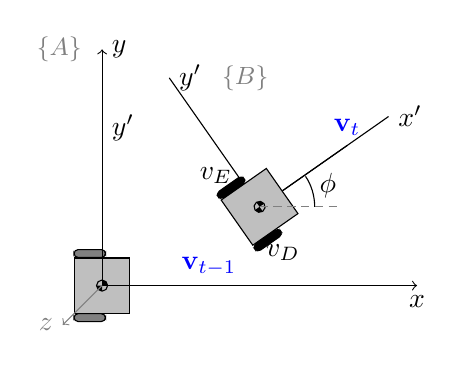
\begin{tikzpicture}[
    force/.style={>=latex,draw=blue,fill=blue},
    axis/.style={densely dashed,gray,font=\small},
    M/.style={rectangle,draw,fill=lightgray,minimum size=0.7cm,thin},
    m/.style={rectangle,draw=black,fill=lightgray,minimum size=0.3cm,thin},
    plane/.style={draw=black,fill=blue!10},
    string/.style={draw=red, thick},
    pulley/.style={thick},
    wheel/.style={fill=black, rounded corners=1.5pt},
]
     \begin{scope}[rotate=0]
        \node[M,transform shape] (M) at (-2,-1) {\centerofmass};
        % Draw axes and help lines
        {[axis,->]
            \draw (M) -- ++(0,2) node(y1_axis)[right] {$y'$};
        }
        % Forces
        {[force,->]
            % Assuming that Mg = 1. The normal force will therefore be cos(alpha)
            \draw (M.east) -- ++(1,0) node[above, blue] {$\mathbf{v}_{t-1}$};
        }
        \draw[wheel, fill=gray] (M.south west) rectangle ++(.4,-.1) node[]{};
        \draw[wheel, fill=gray] (M.north west) rectangle ++(.4,.1)  node[]{};
    \end{scope}


    %% Free body diagram of M
    \begin{scope}[rotate=\iangle]
        \node[M,transform shape] (M) {\centerofmass};
        % Draw axes and help lines
        {[axis,->]
            \draw (M) -- ++(0,2) node(y1_axis)[right] {$y'$};
            \draw (M) -- ++(2,0) node[right] {$x'$};
            % Indicate angle. The code is a bit awkward.
            \draw[solid,shorten >=0.5pt] (\down-\iangle:\arcr)
                arc(\down-\iangle:\down:\arcr);
            \node at (\down-0.5*\iangle:1.3*\arcr) {$\phi$};
        }
        % Forces
        {[force,->]
            % Assuming that Mg = 1. The normal force will therefore be cos(alpha)
            \draw (M.east) -- ++(1,0) node[above, blue] {$\mathbf{v}_t$};
        }
        \draw[wheel] (M.south west) rectangle ++(.4,-.1) node[below]{$v_D$};
        \draw[wheel] (M.north west) rectangle ++(.4,.1)  node[left]{$v_E$};
    \end{scope}
    % Draw gravity force. The code is put outside the rotated
    % scope for simplicity. No need to do any angle calculations. 
    \draw[axis,] (M.center) -- ++(1,0) node[below] {};
    %%
    \node[right, gray,font=\small, xshift=8] at (y1_axis) {$\{B\}$};
    %%
    \draw[, ->] (-2,-1) -- ++(4,0) node[below] {$x$};
    \draw[, ->] (-2,-1) -- ++(0,3) node(y_axis)[right] {$y$};
    \draw[gray, ->] (-2,-1) -- ++(-.5,-.5) node[left] {$z$};
    \node[left, gray,font=\small, xshift=-10] at (y_axis) {$\{A\}$};
\end{tikzpicture}

    \caption{Robô - Dois Graus de Liberdade}
    \label{fig:car01}
    \end{figure}

\subsection{Robô Omnidirecional}
\subsection{Robô Com Esteira}


\section{Dinâmica com Restrições de Movimento}

Tipicamente, um robô com rodas apresenta uma série de restrições relacionadas ao seu modelo de construção, tais restrição tem origem em limitações impostas pelas leis da cinemática e dinâmica.

As restrições dinâmicas têm origem proposta de modelo dinâmico do sistema, onde as limitação se apresentam devido a fatores como a inércia ou mesmo restrições nos atuadores \cite{klancar2017wheeled}.

Do lado da cinemática, as restrições estão relacionadas com a construção do robô e seu modelo cinemático. Podemos classificar as restrições cinemática, sendo elas holonômicas ou não holonômicas. Restrições holonômicas estão relacionadas a dimensionalidade da descrição do estado de um sistema, sendo ele expresso em coordenadas generalizadas, conforme demonstrado em Fig. \ref{fig:2dof-robot}.

Um sistema é considerado holonômico se não tiver restrições holonômicas, não apresentando assim, limitação em seu espaço de velocidades e portanto, todas as direções de movimento de espaço são possíveis. Neste aspecto, podemos considerar o Robô de dois graus de liberdade da Fig. \ref{fig:2dof-robot}, um sistema holonômico, caso não haja restrição da base do robô em $\theta_1$.

Já em um sistema não holonômico, tais restrições impedem que o robô, mova em direções arbitrárias. Um exemplo clássico é apresentado na Fig. \ref{fig:car01}, onde o robô diferencial possui restrições ao movimento em $y'$.




\subsection{Restrições Holonômicos}
 Um sistema holonômico possui restrições que dependem das coordenadas generalizadas, como já foi visto acima. Para tais sistemas com $n$ coordenadas generalizadas $\mathbf{q} = [q_1, \cdots, q_n]$, temos a seguinte equação que expressa tais restrições.

 \begin{equation}
     f(\mathbf{q}) = f(q_1, \cdots, q_n) = 0
     \label{eq:homo}
 \end{equation}

 onde a função $f$ e sua derivada são funções contínuas.

 Observa-se também que a função da equação Eq. \ref{eq:homo} não depende das velocidades ou de qualquer derivada de ordem superior com relação a $t$.

 Em geral, podemos ter $m$ restrições holonômicas, ou seja $(m<n)$.




 Equilíbrio de Energias - Formulação de Lagrange:

 \begin{equation}
     \mathcal{L}= \mathcal{T} - \mathcal{V}
 \end{equation}

A equação de energia cinética ($\mathcal{T}$) é dada por:

\begin{equation}
   \mathcal{T} = \frac{1}{2} \sum\limits_{k=1}^{N}{\mathbf{\dot{q}}_k}^T  \mathbf{M}_k {\mathbf{\dot{q}}_k}+ \frac{1}{2} \sum\limits_{k=1}^{N}\mathbf{\omega}_k^T \mathbf{J}_k \mathbf{\omega}_k
\end{equation}

A equação de Energia Potencial Gravitacional($\mathcal{V}_g$) é dada por\footnote{Depende do típo de energia potencial do sistema, neste caso - gravitacional}

\begin{equation}
   \mathcal{V}_g = \sum\limits_{k=1}^{N}\mathbf{M}g\Delta \underbrace{y_k}_{\text{altura}}
\end{equation}  


\begin{tabular}{l|l}
    $\mathbf{M}$               & Massa              \\
    $\mathbf{\omega}$ & Velocidade Angular \\
    $\mathbf{J}$               & Inércia         \\
\end{tabular}


Para Sistemas Holonômicos:
\begin{equation}
    \frac{d}{\df{t}}\left( \parcial{}{\mathcal{L}}{\dot{q}_k}\right)
    -\parcial{}{\mathcal{L}}{q_k}
    = f_k, \quad k = 1,2,...,n
\end{equation}


onde $k$ é o index das coordenadas generalizadas de $g_k$, $f_k$ são as forças externas que agem no sistema .

O modelo dinâmico de um robô movel sem restrições de movimento pode ser expresso pelo sistema de matrizes abaixo:

\begin{equation}
    \mathbf{M(q)\ddot{q}+ C(q, \dot{q})+ \color{red}{F(\dot{q})}\color{gray}+G(q) = E(q)u}
\end{equation}

onde, 
\begin{tabular}{ r | l }
  $\mathbf{q}$               & Vetor das coordenadas generalizadas   \\
  $\mathbf{M(q)}$            & Matriz de massa e inercia             \\
  $\mathbf{C(q, \dot{q})}$   & Vetor de força Coriolis e centrifuga  \\
  $\color{red}{\mathbf{F(\dot{q})}}$      & Vetor de atrito, força não conservativa\footnotemark\\
  $\mathbf{G(q)}$            & Vector da força gravitacional         \\
  $\mathbf{E(q)}$            & Matriz dos tranformação dos atuadores \\
  $\mathbf{u}$               & Vetor de entrada                      \\
\end{tabular}

\footnotetext{As forças que não fazem parte do balanço de energia no formalismo de lagrange, devem ser adicionadas a posteriori no sistema de equações}

A solução numérica pode ser dada através da integração da aceleração ($\mathbf{\ddot{q}}$):

\begin{equation}
    \mathbf{\ddot{q}}=\mathbf{M(q)}^{-1}\left\{\mathbf{-C(q, \dot{q})-F(\dot{q})-G(q) + E(q)u}\right\}
\end{equation}

Dito isso, usaremos o exemplo do braço robótico da Fig. \ref{fig:2dof-robot} para exrpressar o sistema em equações de estado, conforme a código abaixo:

\begin{equation*}
    \mathbf{X} = 
    \begin{bmatrix}
        \mathbf{q_1 q_2, \dot{q}_1, \dot{q}_2}.  
    \end{bmatrix}
\end{equation*}

\begin{lstlisting}[language=Python]
    def robot2dof(t,X):
        q1  = X[0]
        q2  = X[1]
        dq1 = X[2] 
        dq2 = X[3]
        # Inertial matrix
        Mq = np.array([...]) 
        # C Matrix
        Cq = np.array([...])
        # Gravitational matrix 
        Gq = np.array([...])
        # Friction Force
        ks = 0
        Fa = ks * np.array([[dq1],[dq1]])
        # Atuator
        U_gain =  tau1 = tau2 = 0
        Eu = U_gain * np.array([[tau1],[tau2]])
        # Init Model
        xdot = np.zeros(4,)
        
        #dinamic
        q2dot = inv(Mq).dot(-Cq-Fa-Gq)
        # states
        xdot[0] = dq1
        xdot[1] = dq2
        xdot[2] = q2dot[0]
        xdot[3] = q2dot[1]

        return xdot
\end{lstlisting}

\subsection{Sistemas Não-Holonômicos}


\section{Modelagem de Robô Móvel com restrições de Movimento}


\begin{figure}
    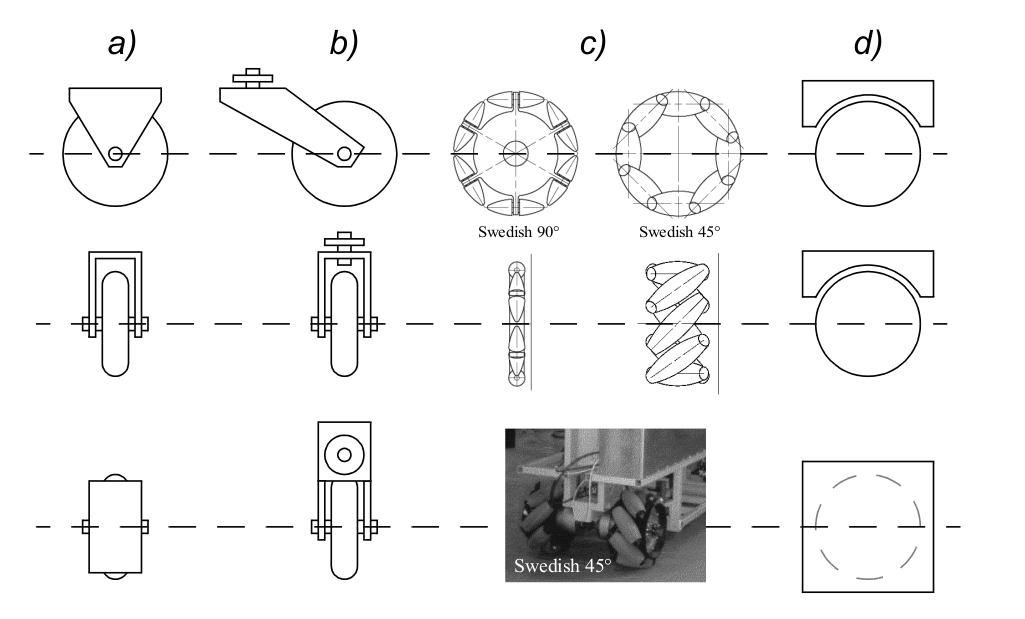
\includegraphics[width=0.8\textwidth]{chapters/chapter1/figures/tipo_de_rodas.png}
    % \cite{siegwart2011introduction}
    \caption{ (a) Standard wheel: two degrees of freedom. (b) castor wheel. (c) Swedish wheel: three degrees of freedom. (d) Ball or spherical wheel: realization technically difficult.}
\end{figure}


 Restrição não-holonômica

 O robô pode mover-se apenas na direção normal ao eixo das rodas motrizes


\begin{equation*}
    \dot{x}\sin(\phi) - \dot{y}\cos(\phi) = 0
\end{equation*}

As próprias rodas já inserem as restrições!


\begin{figure}
    \def\iangle{35} % Angle of the inclined plane
\def\down{0}
\def\arcr{0.7cm} % Radius of the arc used to indicate angles
\newcommand\centerofmass{%
    \tikz[radius=0.2em] {%
        \fill (0,0) -- ++(0.2em,0) arc [start angle=0,end angle=90] -- ++(0,-0.4em) arc [start angle=270, end angle=180];%
        \draw (0,0) circle;%
    }%
}

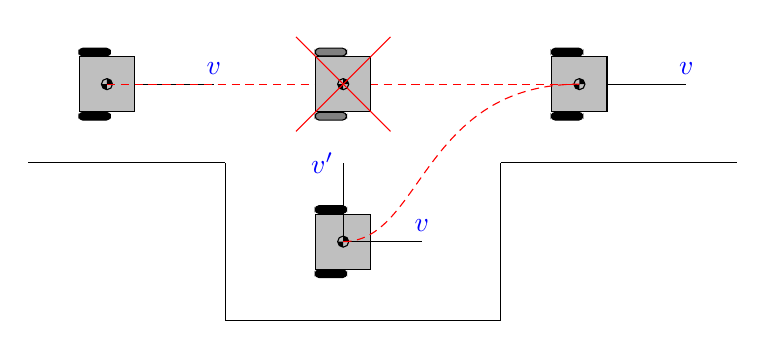
\begin{tikzpicture}[
    force/.style={>=latex,draw=blue,fill=blue},
    axis/.style={densely dashed,gray,font=\small},
    M/.style={rectangle,draw,fill=lightgray,minimum size=0.7cm,thin},
    m/.style={rectangle,draw=black,fill=lightgray,minimum size=0.3cm,thin},
    plane/.style={draw=black,fill=blue!10},
    string/.style={draw=red, thick},
    pulley/.style={thick},
    wheel/.style={fill=black, rounded corners=1.5pt},
]
     \begin{scope}[rotate=0]
        \node[M,transform shape] (M1) at (0,0) {\centerofmass};
        % Draw axes and help lines
        % Forces
        {[force,->]
            % Assuming that Mg = 1. The normal force will therefore be cos(alpha)
            \draw (M1.east) -- ++(1,0) node[above, blue] {$v$};
        }

        \draw[wheel,] (M1.south west) rectangle ++(.4,-.1) node[]{};
        \draw[wheel,] (M1.north west) rectangle ++(.4,.1)  node[]{};
    \end{scope}


    \begin{scope}[rotate=0]
        \node[M,transform shape] (M2) at (6,0) {\centerofmass};
        % Draw axes and help lines
        % Forces
        {[force,->]
            % Assuming that Mg = 1. The normal force will therefore be cos(alpha)
            \draw (M2.east) -- ++(1,0) node[above, blue] {$v$};
        }

        \draw[wheel,] (M2.south west) rectangle ++(.4,-.1) node[]{};
        \draw[wheel,] (M2.north west) rectangle ++(.4,.1)  node[]{};
    \end{scope}
    \begin{scope}[rotate=0]
        \node[M,transform shape] (M3) at (3,-2) {\centerofmass};
        % Draw axes and help lines
        % Forces
        {[force,->]
            % Assuming that Mg = 1. The normal force will therefore be cos(alpha)
            \draw (M3.center) -- ++(1,0) node[above, blue] {$v$};
            \draw (M3.center) -- ++(0,1) node[left, blue] {$v'$};
        }

        \draw[wheel,] (M3.south west) rectangle ++(.4,-.1) node[]{};
        \draw[wheel,] (M3.north west) rectangle ++(.4,.1)  node[]{};
    \end{scope}

%%
    \draw (-1,-1)           -- ++(2.5,0) node[](wall_1){};
    \draw (wall_1.center)   -- ++(0,-2) node[](wall_2){};
    \draw (wall_2.center)   -- ++(3.5,0) node[](wall_3){};
    \draw (wall_3.center)   -- ++(0,2) node[](wall_4){};
    \draw (wall_4.center)   -- ++(3,0) node[](wall_4){};    

    \pausar
    \draw[densely dashed, red] (M1.center) -- (M2.center);
    
    \pausar

    \begin{scope}[rotate=0]
        \node[M,transform shape] (M4) at (3,0) {\centerofmass};
        % Draw axes and help lines
        % Forces

        \draw[wheel,fill=gray] (M4.south west) rectangle ++(.4,-.1) node[]{};
        \draw[wheel,fill=gray] (M4.north west) rectangle ++(.4,.1)  node[]{};

        \draw[red] (3,0) -- ++(-0.6,-0.6) node[]{};
        \draw[red] (3,0) -- ++(0.6,-0.6) node[]{};
        \draw[red] (3,0) -- ++(-0.6,0.6) node[]{};
        \draw[red] (3,0) -- ++(0.6,0.6) node[]{};
    \end{scope}

    \draw[densely dashed, red] (M3.center) .. controls ++(1,0) and ++(-2,0) .. (M2.center);

    % Draw gravity force. The code is put outside the rotated
    % scope for simplicity. No need to do any angle calculations. 
\end{tikzpicture}

\end{figure}


\begin{figure}
    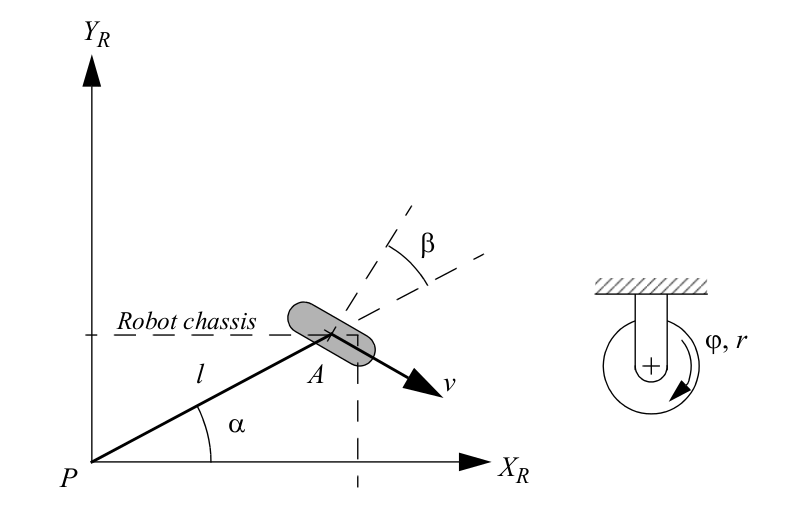
\includegraphics[width=0.6\textwidth]{chapters/chapter1/figures/wheels_const.png}    
    \caption{A fixed standard wheel and its parameters.}
\end{figure}










Restrições - Robô Diferencial

\def\iangle{35} % Angle of the inclined plane
\def\down{0}
\def\arcr{0.7cm} % Radius of the arc used to indicate angles
\newcommand\centerofmass{%
    \tikz[radius=0.2em] {%
        \fill (0,0) -- ++(0.2em,0) arc [start angle=0,end angle=90] -- ++(0,-0.4em) arc [start angle=270, end angle=180];%
        \draw (0,0) circle;%
    }%
}

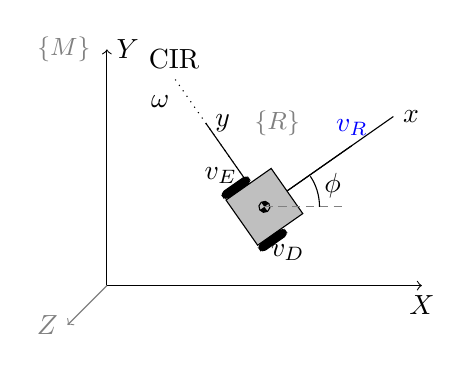
\begin{tikzpicture}[
    force/.style={>=latex,draw=blue,fill=blue},
    axis/.style={densely dashed,gray,font=\small},
    M/.style={rectangle,draw,fill=lightgray,minimum size=0.7cm,thin},
    m/.style={rectangle,draw=black,fill=lightgray,minimum size=0.3cm,thin},
    plane/.style={draw=black,fill=blue!10},
    string/.style={draw=red, thick},
    pulley/.style={thick},
    wheel/.style={fill=black, rounded corners=1.5pt},
]
    %% Free body diagram of M
    \begin{scope}[rotate=\iangle]
        \node[M,transform shape] (M) {\centerofmass};
        % Draw axes and help lines
        {[axis,->]
            \draw (M) -- ++(0,1.3) node(y1_axis)[right] {$y$};
            \draw (M) -- ++(2,0) node[right] {$x$};
            % Indicate angle. The code is a bit awkward.
            \draw[solid,shorten >=0.5pt] (\down-\iangle:\arcr)
                arc(\down-\iangle:\down:\arcr);
            \node at (\down-0.5*\iangle:1.3*\arcr) {$\phi$};
        }
        % Forces
        {[force,->]
            % Assuming that Mg = 1. The normal force will therefore be cos(alpha)
            \draw (M.east) -- ++(1,0) node[above, blue] {$v_R$};
        }
        \draw[wheel] (M.south west) rectangle ++(.4,-.1) node[below]{$v_{D}$};
        \draw[wheel] (M.north west) rectangle ++(.4,.1)  node[left]{$v_{E}$};
        \draw [dotted, -](M) -- ++(0,2) node(CIR)[above] {CIR};
        \node[below,  yshift=-10, xshift=-5] at (CIR) {$\omega$};
    \end{scope}
    % Draw gravity force. The code is put outside the rotated
    % scope for simplicity. No need to do any angle calculations. 
    \draw[axis,] (M.center) -- ++(1,0) node[below] {};
    %%
    \node[right, gray,font=\small, xshift=8] at (y1_axis) {$\{R\}$};
    %%
    \draw[, ->] (-2,-1) -- ++(4,0) node[below] {$X$};
    \draw[, ->] (-2,-1) -- ++(0,3) node(y_axis)[right] {$Y$};
    \draw[gray, ->] (-2,-1) -- ++(-.5,-.5) node[left] {$Z$};
    \node[left, gray,font=\small, xshift=-10] at (y_axis) {$\{M\}$};
\end{tikzpicture}

\begin{equation}
    \mathbf{A} = 
    \begin{bmatrix}
        -\sin(\phi) & \cos(\phi) & 0
    \end{bmatrix}
\end{equation}


Equilíbrio de Energias:

\begin{equation}
    \mathcal{L}= \mathcal{T} - \mathcal{V}
\end{equation}

A equação de energia cinética ($\mathcal{T}$) é dada por:

\begin{equation}
    \mathcal{T} = \sum\limits_{i=0}^{N-1} \frac{1}{2} {}_{i}^{i+1}\dot{\mathbf{P}}^T\cdot m_{i}\cdot {}_{i}^{i+1}\dot{\mathbf{P}}+ \mathbf{\omega}_i^T\cdot \mathbf{J}_i \cdot \mathbf{\omega}_i
\end{equation}

ou para um robô em uma superfície:

\begin{equation*}
    \boxed{
        \mathcal{T} = \frac{m}{2}\left(\dot{x}^2+\dot{y}^2 \right)+ \frac{J}{2}\dot{\phi}^2}
    \text{, e  }
    \boxed{\mathcal{V} = 0}
\end{equation*}
               
    onde:
    \begin{tabular}{l|l}
        $m$               & Massa              \\
        $\mathbf{\omega}$ & Velocidade Angular \\
        $J$               & Inércia            \\
    \end{tabular}
              

Formulação de Lagrange

Para Sistemas Holonômicos:

\begin{equation}
    \frac{d}{\df{t}}\left( \parcial{}{\mathcal{L}}{\dot{q}_k}\right)
    -\parcial{}{\mathcal{L}}{q_k}
    +\tau_{d_k}
    = f_k, \quad k = 1,2,...,n
\end{equation}

Para Sistemas Não-Holonômicos \footnote{onde $k$ é o index das coordenadas generalizadas de $g_k$, $P$ representas as energias dissipativas (Atrito),
$\tau_d$ representa qualquer disturbio no sistema, $f_k$ são as forças externas que agem no sistema e $a_{jk}$ são os coeficientes das restrições de movimento.}
\begin{equation}
    \frac{d}{\df{t}}\left( \parcial{}{\mathcal{L}}{\dot{q}_k}\right)
    -\parcial{}{\mathcal{L}}{q_k}
    +\tau_{d_k}
    = f_k - \sum\limits^{m}_{j=1}\lambda_j a_{jk}
\end{equation}

O modelo dinâmico de um robô movel com restrições de movimento pode ser expresso pelo sistema de matrizes abaixo:

\begin{equation}
    \mathbf{M(q)\ddot{q}+ C(q, \dot{q})+ F(\dot{q})+G(q) = E(q)u -A}^T\mathbf{(q)}\boldsymbol{\lambda}
\end{equation}

onde:
\begin{tabular}{ r | l }
    $\mathbf{q}$               & Vetor das coordenadas generalizadas   \\
    $\mathbf{M(q)}$            & Matriz de massa e inercia             \\
    $\mathbf{C(q, \dot{q})}$   & Vetor de força Coriolis e centrifuga  \\
    $\mathbf{F(\dot{q})}$      & Vetor de atrito                       \\
    $\mathbf{G(q)}$            & Vector da força gravitacional         \\
    $\mathbf{E(q)}$            & Matriz dos tranformação dos atuadores \\
    $\mathbf{u}$               & Vetor de entrada                      \\
    $\mathbf{A}^T\mathbf{(q)}$ & Matriz de restrições de movimento     \\
    $\boldsymbol{\lambda}$     & Multiplicador de Lagrange             \\
\end{tabular}


A solução para $\lambda_i$ pode ser encontrada por:
\begin{itemize}
    \item Método 1: Pseudo-velocidades
    \item Método 2: Redução de Order 
    \item Método 3: Equações de Euler-Lagrange Modificadas 
    \item Método 4: Calculo das Forças de restrições 
\end{itemize}


Formulação de Lagrange - Pseudo-velocidades

O objetivo é resolver as restrições de $\lambda_i$:

\begin{equation}\label{eq:rmrestri}
    \mathbf{M(q)\ddot{q}+ C(q, \dot{q})+ F(\dot{q})+G(q) = E(q)u} - \textcolor{red}{\cancel{\mathbf{A}\mathbf{(q)}^T\boldsymbol{\lambda}}}
\end{equation}

reelembrando:

\begin{equation*}
    \mathbf{\dot{q}} = \mathbf{S}(q)\mathbf{v}
\end{equation*}

bem como:

\begin{equation}\label{eq:aprox_accel}
    \mathbf{\ddot{q}} = \mathbf{\dot{S}}(q)\mathbf{v} + \mathbf{S}(q)\mathbf{\dot{v}}
\end{equation}

Subustituindo \eqref{eq:rmrestri} em \eqref{eq:aprox_accel} e aplicando a relãção $\mathbf{A}(q)\mathbf{S}(q)=0$, temos a equação de aceleração do sistema:

\begin{equation}\label{eq:pseudovelo}
    \mathbf{\dot{v}} = \mathbf{\tilde{M}}^{-1}\left(\mathbf{\tilde{E}u - \tilde{V}} \right)
\end{equation}


Formulação de Lagrange - Pseudo-velocidades

\eqref{eq:pseudovelo} na forma de equação:

\begin{equation*}
    \mathbf{\dot{x}} =
    \begin{bmatrix}
        \mathbf{S}(q)\mathbf{v} \\
        \mathbf{-\tilde{M}}^{-1}\mathbf{\tilde{V}}
    \end{bmatrix}
    +
    \begin{bmatrix}
        \mathbf{0} \\
        \mathbf{\tilde{M}}^{-1}\mathbf{\tilde{E}}
    \end{bmatrix} \mathbf{u}
\end{equation*}

onde:

\begin{equation*}
    \begin{split}
        \mathbf{\tilde{V}} & =
        \mathbf{S}(q)^T\mathbf{M}\mathbf{\dot{S}}(q)\mathbf{v} + \mathbf{S}(q)^T (\mathbf{V + F + G})\\
        \mathbf{\tilde{M}} & = \mathbf{S}(q)^T\mathbf{M}\mathbf{S}(q)\\
        \mathbf{\tilde{E}} & = \mathbf{S}(q)^T\mathbf{E}\mathbf{S}
    \end{split}
\end{equation*}

onde:
\begin{tabular}{ r | l }
    $\mathbf{x}$ & Vetor de estados \\
    $\mathbf{S}$ & Matriz Jacobiana \\
\end{tabular}







% \section{Glossary}
% \begin{Glossary}
% \item[360 Degree Review] Performance review that includes feedback from superiors, peers, subordinates, and clients.
% \item[Abnormal Variation] Changes in process performance that cannot be accounted for by typical day-to-day variation. Also referred to as
% non-random variation.
% \item[Acceptable Quality Level (AQL)] The minimum number of parts that must comply with quality standards, usually stated as a percentage.
% \item[Activity] The tasks performed to change inputs into outputs.
% \item[Adaptable] An adaptable process is designed to maintain effectiveness and efficiency as requirements change. The process is
% deemed adaptable when there is agreement among suppliers, owners, and customers that the process will meet
% requirements throughout the strategic period.
% \end{Glossary}



